\section{React Native CLI}
\textbf{Wichtig}: In der Installationsanleitung auf der Webseite von \textbf{React Native} kann man sein
aktuelles Betriebssystem und seine gewünschte Zielplattform auswählen. Apple erlaubt nicht die
Entwicklung von Apps auf anderen Betriebssystemen als MacOS selbst, d.h. die Entwicklung der iOS-App
ist auf Windows 11, meinem Betriebssystem, nicht möglich. Ich hatte während der Entwicklung nie
Zugriff auf einen PC mit MacOS, daher wurde die gesamte App ausschließlich für Android entwickelt.
Doch sollten wir jemals diese App wirklich veröffentlichen wollen, so wird das Umschreiben keinen
großen Aufwand darstellen, da ich immer darauf geachtet habe, nur Bibliotheken zu verwenden, die
auch für iOS kompatibel sind.

\subsection{Abhängigkeiten und Erstellung des Projekts}
Für die Verwendung der React-Native-CLI werden einige andere Softwarepakete benötigt, darunter --
natürlich -- \underline{\nameref{nodejs}}, mindestens Version 12. Außerdem wird benötigt:

\begin{itemize}
  \item Java SE Development Kit (mind. Version 11)
  \item Android Studio
  \begin{itemize}
    \item Android SDK 11 (R)
    \item Android SDK Platform: API Level 30
    \item Android Virtual Device: Google Pixel 2 mit Android 11
  \end{itemize}
\end{itemize}

Sobald alle Abhängigkeiten installiert wurden, führt man folgenden Befehl aus, um ein neues React
Native Projekt zu erstellen:

\begin{code}[htp]
\begin{lstlisting}[firstnumber=1,language=JavaScript, style=CMD]
C:\example> npx react-native init reactNativeInit
\end{lstlisting}
\caption{CMD - React Native CLI init}
\end{code}

\textbf{NPX} ist ein Befehl, der seit Version 5.2.0 in \textbf{NPM} enthalten ist. Er ist speziell bei CLIs hilfreich,
denn anstatt das Paket react-native auf dem PC zu installieren und dann aufzurufen, wird mit dem
Befehl automatisch die neueste Version der CLI von einem Server abgefragt und ausgeführt. So kann
man sicherstellen, dass niemals eine veraltete Version der CLI verwendet wird.

\newpage

\subsection{Ordnerstruktur}

\subsubsection{Ordner}

% \begin{figure}[H]
%   \begin{center}
%     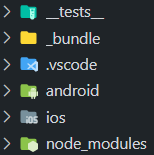
\includegraphics[width=0.5\textwidth]{Theorie/ReactNative/ReactNativeFolders.png}
%     \caption{Ordnerstruktur React Native Init}
%   \end{center}
% \end{figure}

\begin{itemize}
\item \textbf{\_\_tests\_\_/}:\\
In diesem Ordner werden Skripts abgespeichert, die die Funktionalität der App überprüfen sollen,
sogenannte Tests. React Native empfiehlt hierbei die Bibliothek \textbf{Jest}, welche die Durchführung von
Snapshot-Tests ermöglicht. Diese testen, ob sich die Benutzeroberfläche auch so verhaltet, wie
erwartet. Tests sind in großen Projekten nicht mehr wegzudenken, bei kleineren Projekten sind sie
aber meist den Schreibaufwand nicht wert.

\item \textbf{.vscode/}:\\
In diesem Ordner ist es möglich Einstellungen und Skripts für den Text-Editor \textbf{Visual Studio Code}
abzuspeichern, den wir durchwegs für die gesamte Diplomarbeit verwendet haben.

\item \textbf{android/}:\\
Manche Änderungen kann man nicht mit Hilfe von JavaScript vornehmen, manchmal muss man auch die
plattformspezifischen Dateien der App verändern. Diese sind alle im Ordner android vorhanden. In ihm
sind hauptsächlich Konfigurationsdateien für das Build-Automatisierungstool \textbf{Gradle} und Manifest-
Dateien, welche Metadaten zur App enthalten und auch für andere Bibliotheken bearbeitet werden
müssen, z.B. Google-Maps-Funktionalität.

\item \textbf{node\_modules/}:\\
Im Ordner \textbf{node\_modules} werden alle Bibliotheken abgespeichert, die mit Hilfe des Paketmanagers
in das Projekt eingebunden wurden.

\item \textbf{\_bundle/, ios/}:\\
Hier befinden sich lediglich Dateien, welche für das Entwickeln der iOS-App wichtig sind. Bei
unserer Diplomarbeit wurden diese Ordner nicht benötigt.

\end{itemize}

\newpage
\subsubsection{Dateien}
% \begin{figure}[H]
%   \begin{center}
%     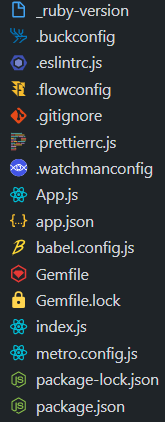
\includegraphics[width=0.5\textwidth]{Theorie/ReactNative/ReactNativeFiles.png}
%     \caption{Dateien React Native Init}
%   \end{center}
% \end{figure}

\begin{itemize}
\item \textbf{index.js, App.js}:\\
\textbf{index.js} ist, wie der Name schon vermuten lässt, die Einstiegsdatei für das Projekt. In ihr wird
nur die Datei \textbf{App.js} eingebunden.

\textbf{App.js} ist also die erste richtige Code-Datei, welche von uns bearbeitet wird. Als Erklärung zeige
ich hier ein klassisches Hallo-Welt-Programm, welches eigentlich von der Expo-CLI erstellt wird,
jedoch sehr gut zur Veranschaulichung dient.

\begin{code}[htp]
\begin{lstlisting}[firstnumber=1,language=JavaScript, style=JSX]
import { StyleSheet, Text, View } from 'react-native';

function App() {
  return (
    <View style={styles.container}>
      <Text>Open up App.js to start working on your app!</Text>
    </View>
  );
}

const styles = StyleSheet.create({
  container: {
    flex: 1,
    backgroundColor: '#fff',
    alignItems: 'center',
    justifyContent: 'center',
  },
});

export default App;
\end{lstlisting}
\caption{React Component - App.js}
\end{code}

In der ersten Zeile des Programms werden diverse React Native Core Components importiert. Core
Components sind, wörtlich übersetzt, die Kernkomponenten des Frameworks, mit ihnen wird der Großteil
der Benutzeroberfläche aufgebaut. Wie bereits erwähnt, werden die React Native Komponenten beim
Kompilieren in die richtigen Komponenten für das Zielsystem umgewandelt.


\begin{figure}[H]
  \begin{center}
    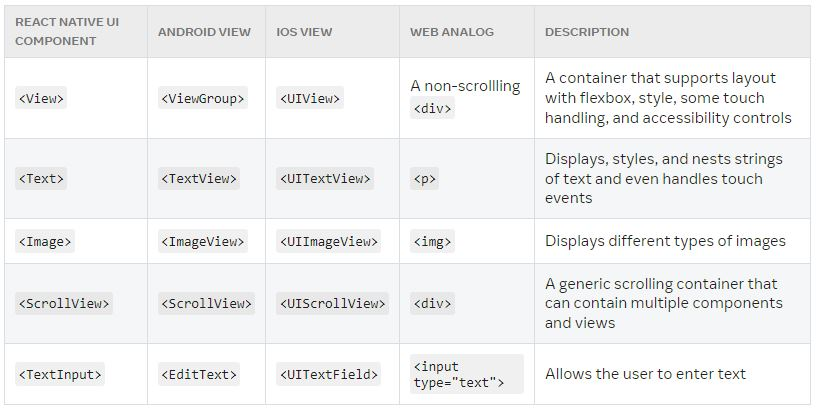
\includegraphics[width=0.9\textwidth]{Mobile/React Native CLI/CoreComponents.JPG}
    \caption{Tabelle - Core Components und deren Gegenstücke \cite{reactNativeCoreComponents}}
  \end{center}
% \begin{table}[H]
% \centering
% \begin{tabular}{|l|l|l|l|}
%   \hline
%   \textbf{Komponente} & \textbf{Android} & \textbf{iOS} & \textbf{HTML} \\ \hline\hline
%   View                & ViewGroup        & UIView       & div          \\
%   Text                & TextView         & UITextView   & p            \\ \hline
% \end{tabular}
% \end{table}
\end{figure}

In der nächsten Zeile wird unserer erster React-Component erzeugt, welcher im Grunde nur eine
Funktion ist, die \underline{\nameref{jsx}}-Code als Rückgabewert liefert.

In Zeile 5 wird zur View ein React Native \textbf{StyleSheet} zugewiesen. Man verwendet nämlich kein
gewöhnliches \underline{\nameref{css}}, wie in der Webentwicklung, sondern ein relativ ähnlich aufgebautes,
eigenes System zur Gestaltung der App. Ein wichtiger Unterschied ist, dass die Attribut-Namen im
\textbf{StyleSheet} nicht durch Bindestriche getrennt, sondern in der LowerCamelCase-Notation geschrieben
werden \cite{camelCaseNotation}.

Am Ende der Datei wird noch die Komponente als Default exportiert, damit sie von \textbf{index.js} verarbeitet
werden kann \cite{jsModules}.

\item \textbf{app.json, package.json}:\\
\textbf{app.json} wird von React Native generiert und enthält zu Beginn bloß den Namen und Anzeigenamen der
App.

% \begin{figure}[H]
%   \begin{center}
%     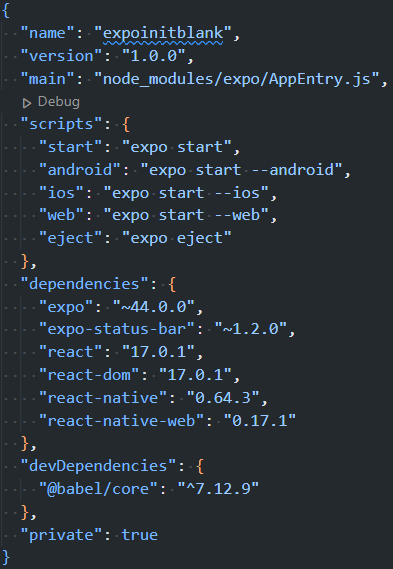
\includegraphics[width=0.5\textwidth]{Theorie/ReactNative/package-json.png}
%     \caption{package.json Inhalt}
%   \end{center}
% \end{figure}

\textbf{package.json} hat einen ähnlichen Zweck, auch darin sind Name, Versionsnummer, aber auch der
Eintrittspunkt in die App abgespeichert. In Scripts werden Kommandozeilenbefehle abgespeichert, die
mit Hilfe des Befehls \textbf{npm run <script>} aufgerufen werden können. Im nächsten Objekt werden die
Namen der Bibliotheken aufgelistet, welche für das Ausführen der App benötigt werden. Bibliotheken,
die nur während der Entwicklung benötigt werden, sind unter devDependencies abzuspeichern (beim
Installieren den Tag \textbf{-{}-save-dev} anhängen).

\item \textbf{package-lock.json}:\\
\textbf{package-lock.json} gehört zu \textbf{NPM} und ist eine Lockfile. In einer Lockfile werden alle installierten
Dependencies noch einmal aufgelistet und mit der Versionsnummer abgespeichert, um sicherzugehen,
dass bei der Generierung von \textbf{node\_modules/} alle Bibliotheken immer dieselbe Version haben.

\newpage

\item \textbf{babel.config.js}:\\
\textbf{Babel} ist ein sogenannter JavaScript-Transpiler. Er wandelt JavaScript-Features, welche erst in
späteren Versionen des \textbf{ECMAScript}-Standards eingebaut und möglicherweise noch nicht von allen
Systemen unterstützt werden, in JavaScript-Code um, welcher auch von älteren Versionen verstanden
werden kann, um (vgl. ein Compiler wandelt lesbaren Code in Maschinencode um). Außerdem hat er noch
einige andere Funktionen, welche durch Plugins hinzugefügt werden können. In der Konfigurationsdatei
wird nur eine vorgefertigte Liste an Plugins in das Projekt eingebunden, das \textbf{babel-preset-expo}.

\item \textbf{metro.config.js}:\\
Eine Konfigurationsdatei für den JavaScript-Bundler \textbf{Metro}.

\item \textbf{.gitignore}:\\
In die Datei \textbf{.gitignore} fügt man Datei- und Ordnernamen ein, die nicht von der Versionsverwaltung
gesichert werden sollen. Sehr zu empfehlen ist dies beim Ordner \textbf{node\_modules/}, da dieser schon
direkt nach der Erstellung 170 Megabytes groß ist und er aus den Dateien \textbf{package.json} und \textbf{yarn.lock}
generiert werden kann.

\item \textbf{.eslintrc.js}:\\
\textbf{ESLint} ist ein Linter für JavaScript, er überprüft alle vorhandenen JavaScript-Dateien nach
möglichen syntaktischen oder semantischen Fehlern und kann sogar mögliche Verbesserungen vorschlagen.

\item \textbf{.prettierrc.js}:\\
\textbf{Prettier} ist ein Werkzeug, welches jeder Programmierer verwenden sollte. Es übernimmt die Aufgabe
des Formatierens von Quellcode, sodass ein einheitliches System herrscht und Zeit gespart wird.

\item \textbf{.flowconfig}:\\
In JavaScript gibt es, Stand 2022, keine statische Typsicherheit bei Variablen, jede Variable kann
jeden Typ annehmen. \textbf{Flow} ist ein System, welches in Kommentaren in Code die Typen von bestimmten
Variablen festlegt und beim Schreiben der App Fehler anzeigt, falls diese verletzt werden.
Stattdessen könnte man auch die Sprache \textbf{TypeScript} verwenden, welche zu gewöhnlichem JavaScript
kompiliert werden kann.

\item \textbf{.watchmanconfig}:\\
\textbf{Watchman} wurde von Facebook entwickelt, um die Veränderung von Dateien zu registrieren und bestimmte
Prozesse dadurch zu starten, z.B. das Kompilieren von TypeScript zu JavaScript.

\item \textbf{Gemfile, Gemfile.lock}:\\
Diese beiden Dateien werden nur bei der Entwicklung von iOS-Apps benötigt. Sie gehören zum Ruby-
Projekttool \textbf{Bundler}.

\end{itemize}

\newpage
\subsection{Metro}
\label{metrobundler}
Beim Start der App wird als erstes der \textbf{Metro Bundler} initialisiert. Er besteht aus einem Server,
welcher den geschriebenen Code mittels \textbf{Babel} kompiliert und anschließend an die App schickt. Dadurch
verhindert man, jedes mal die App neu auf das Gerät installieren zu müssen, um eine kleine Änderung
im Text sehen zu können. Beim Einbinden von neuen JavaScript-Bibliotheken muss allerdings der
Bundler neu gestartet werden, um diese verwenden zu können.

Um den Server zu starten gibt man folgenden Befehl ein:

\begin{code}[htp]
\begin{lstlisting}[firstnumber=1,language=JavaScript, style=CMD]
C:\example\reactNativeInit> npm start
\end{lstlisting}
\caption{CMD - Kurzschreibweise für den Befehl npm run start}
\end{code}

\begin{figure}[H]
  \begin{center}
    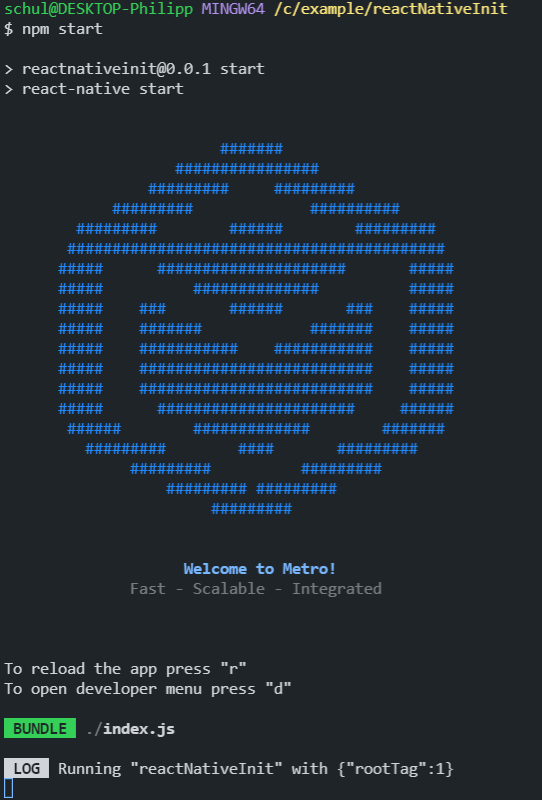
\includegraphics[width=0.5\textwidth]{Theorie/ReactNative/MetroBundler.png}
    \caption{Der Metro-Server in Aktion}
  \end{center}
\end{figure}

\newpage
Als nächstes öffnet man den Ordner \textbf{root/android} in Android Studio. Man hat nun zwei Möglichkeiten,
die App auszuführen:

\begin{enumerate}
  \item Mit einem virtuellen Android Gerät (Android Virtual Device AVD):\\
Dazu öffnet man in Android Studio den AVD-Manager und erstellt einen neuen Emulator mit einer
Android Version von 11. Danach startet man den Emulator und führt folgenden Befehl aus:

\begin{code}[htp]
\begin{lstlisting}[firstnumber=1,language=JavaScript, style=CMD]
C:\example\reactNativeInit> npm run android
\end{lstlisting}
\caption{CMD - Die App wird auf dem Emulator installiert und ausgeführt.}
\end{code}

\begin{figure}[H]
  \begin{center}
    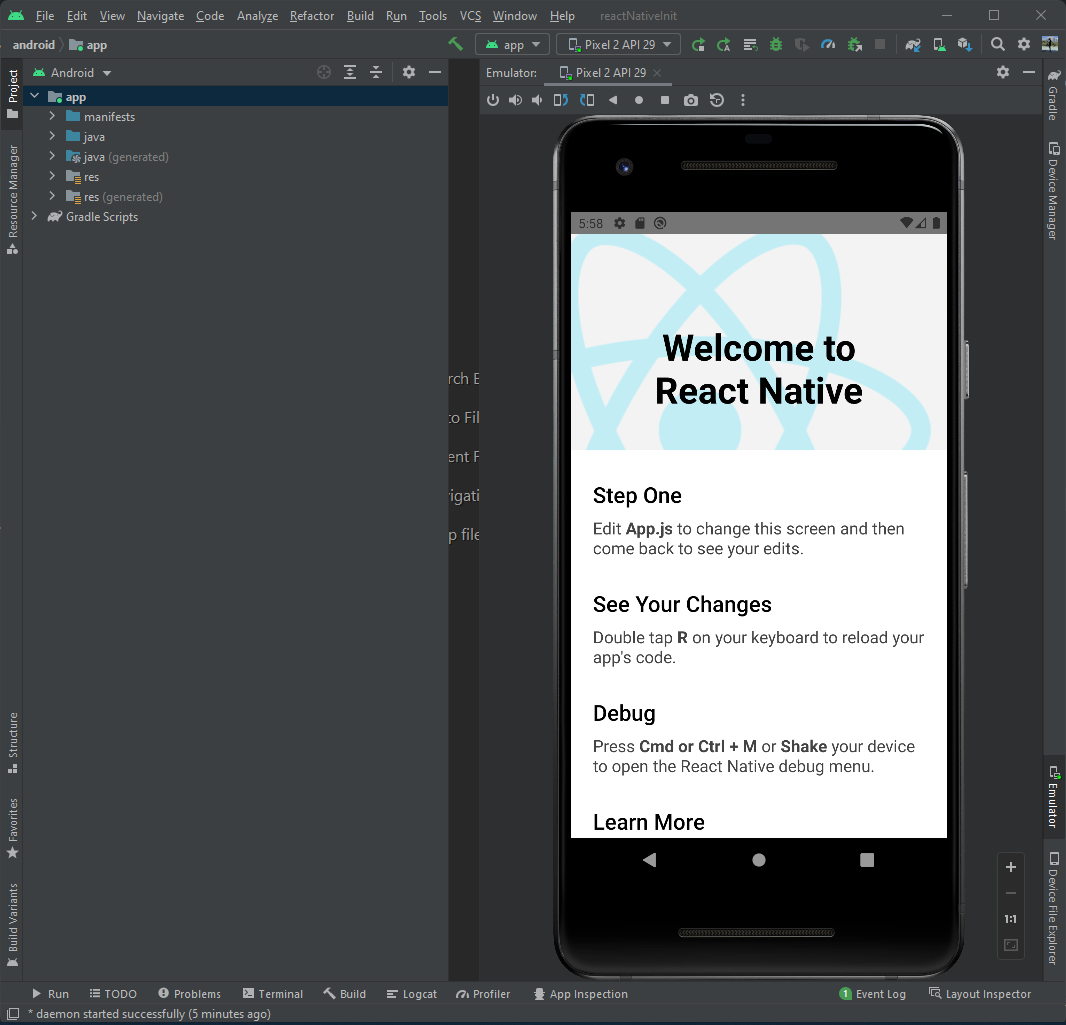
\includegraphics[width=0.8\textwidth]{Theorie/ReactNative/AndroidStudio.png}
    \caption{Die Beispiel-App in Android Studio}
  \end{center}
\end{figure}

\newpage
  \item Mit einem physischen Android-Gerät:\\
Als erstes aktiviert man auf dem Gerät in den Einstellungen USB-Debugging und schließt es per USB an
den PC an. Wenn alle Treiber installiert sind, müsste es dann direkt in Android Studio erkannt
werden, um die App zu installieren.

Jetzt muss noch ein Tunnel über die USB-Verbindung erzeugt werden, damit das Gerät darüber mit dem
lokalen Metro-Server kommunizieren kann. Man listet alle Geräte auf und erzeugt dann mit der
Device-Identifikation einen Tunnel.

\begin{code}[htp]
\begin{lstlisting}[firstnumber=1,language=JavaScript, style=CMD]
C:\example\reactNativeInit> adb devices
List of devices attached
34299o5j85o496g3        device
emulator-8125           device

C:\example\reactNativeInit> adb -s 34299o5j85o496g3 reverse tcp:8081 tcp:8081
8081
\end{lstlisting}
\caption{CMD - Erstellung eines TCP-Tunnels über USB}
\end{code}

\end{enumerate}